
In 1997, Deep Blue, a computer built by IBM won a six games match against the current
chess world champion Garry Kasparov. Humans got beaten on Chess, but remain undefeated in other games. Consequently, researchers are looking for improvements in Artificial Intelligence. We are going to work on it as well.
\newline
\newline
Our project is called Fast and furious game playing, MonteCarlo drift. Our purpose is to create an Artificial Intelligence able to compete against humans using the MonteCarlo Tree Research.
\newline
We will only focus on two players strategy board games. Furthermore, we want to avoid games already solved\footnote{A game solved is a game where good algorithms are able to find the perfect move in each situation to win, or to draw. For instance, \textit{Tic Tac Toe} or \textit{Draughts} are solved games.}. We will choose something not studied entirely. We want to work on some new application. That is why we are interested by Arimaa.
\newline
\newline
For our game, we will need a program and statistics to make a good Artificial Intelligence. To evaluate the best move, the algorithm will just develop a tree by creating nodes composed of all possible moves. Then it will evaluate these nodes making statistics. These statistics can be the result of a deeper exploration of a node, or the result of a loss of an important piece. The algorithm will then be able to choose the best move according to the figures.
\smallbreak
\begin{figure}[!h] 
\centerline{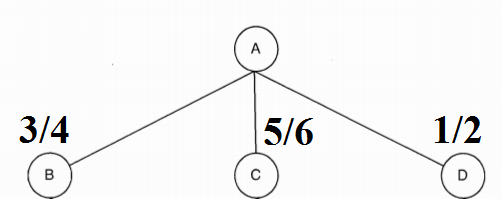
\includegraphics[scale=0.50]{1_Presentation/1.1_Our_project_Dan/tree}}
  \caption{An exploring tree :\newline The probabilities related to the nodes are the numbers, so the best node is the node B according to the statistics. See more in 2.1 part.}
  \centering
\end{figure}
MonteCarlo Tree Research is an algorithm able to take these optimal decisions. It has been used in the past for \textit{Draughts}, or \textit{Chess}. By exploring random numerous possibilities, this algorithm will be able to recognize some of the patterns useful for our Artificial Intelligence.
We will parallelize this algorithm in order to use it in a multi-core machine, to improve his efficiency, and to go deeper into the trees.
With that environnement, we will be able to use MCTS algorithms at his finest.
\newline
\newline
We will analyse parallelization methods, we will present it, and then we will choose the one adapted to our project.
Thanks to the results of these latest methods, we will be able to choose a state resulting of the current move. Then we will explore the tree and with the same methods as before, we will figure out what the opponent will most probably do. The way we will be exploring the tree will only depend on the parallelization method.
The first part of our project will be the analysis of latest thesis of technologies we will use, in order to choose the best one, and using it on the right environment, to improve his  efficiency.
In the next part, we will choose technologies we will need to achieve our goals, we will create a UML diagram to settle down our program.
\newline
\newline
Finally, in the last part, we will implement this program, and its documentation and test his executing on Grid5000, a cluster of multi-core machines.
What is interesting in this project is we will create an Artificial Intelligence using technologies and methods fully optimized. Then we will create a program that can lead to true improvements for current algorithms applied to this game.


